\documentclass[letterpaper, landscape]{exam}
\usepackage{2in1, lscape} 
\printanswers

\usepackage{units} 
\usepackage[fleqn]{amsmath}
\usepackage{float}
\usepackage{mdwlist}
\usepackage{booktabs}
\usepackage{caption}
\usepackage{fullpage}
\usepackage{enumerate}
\usepackage{graphicx}

\setcounter{tocdepth}{1}
\everymath{\displaystyle}

\author{}
\date{\today}
\title{Calculus I \\ Week Five}

\begin{document}

  \maketitle
  \tableofcontents

  \section{Homework Three} 
  \begin{itemize}
    \item sorry about the quantity and the graphing problems
    \item infinite limit vs. limit does not exist
  \end{itemize}

  \section{Continuity Definition}

  A function is continuous at $a$ if:
  \[
    \lim_{x \to a} f(x) = f(a) 
  \]

  \begin{itemize*}
    \item implies $\lim_{x \to a} f(x)$ is defined
    \item implies $f(a)$ is defined
    \item matches intuitive idea for continuous line
    \item can draw graph without lifting pen from paper
    \item draw examples of continuous and discontinuous functions including:
      \begin{itemize*}
        \item $f(x)$ undefined at $a$
        \item hole at $f(a)$ with $f(a)$ defined at a different value
        \item left limit not equal to right limit
      \end{itemize*}

    \item a {\em removable} discontinuity occurs when $f(x)$ is undefined at $a$. It can
      be removed by defining a suitable value for $f(a)$.

  \end{itemize*}

  examples:
  \begin{enumerate}
    \item 
      \[
        f(x) = \frac{1}{x - 1}
      \]
      
      $f(1)$ doesn't exist and $\lim_{x \to 1} f(x)$ also doesn't exist (See Figure
      \ref{fig:ex01}).

      \begin{figure}[H]
        \centering
        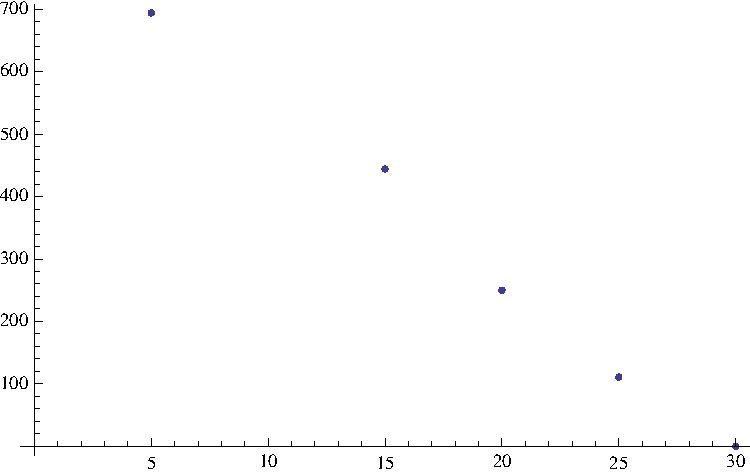
\includegraphics[scale = 0.5]{ex01.pdf}
        \caption{Example 1}
        \label{fig:ex01}
      \end{figure}

    \item 
      \[
        f(x) = \frac{x^2 - 1}{x - 1} = x + 1
      \]
      
      $f(1)$ doesn't exist. This is an example of a {\em removable discontinuity}

    \item
        \[
          f(x) = 
            \begin{cases}
              \frac{x^2 - 1}{x - 1} & \text{if } x \neq 1 \\
              0                     & \text{if } x = 1 \\
            \end{cases}
        \]

        $f(1) \neq\lim_{x \to 1} f(x)$

    \item
        \[
          f(x) = 
            \begin{cases}
              \frac{x^2 - 1}{x - 1} & \text{if } x \neq 1 \\
              2                     & \text{if } x = 1 \\
            \end{cases}
        \]

        continuous

  \end{enumerate}

  \section{Left and Right Continuity}
  
  \begin{description}
    \item[Continuous from the Left] $\lim_{x \to a^-} f(x) = f(a)$ 
    \item[Continuous from the Right] $\lim_{x \to a^+} f(x) = f(a)$ 
  \end{description}

  \section{Continuous on an Interval}
  A function is continuous on an interval if it is continuous at every point in the
  interval.

  \section{Combining Continuous Functions}
  If $f$ and $g$ are continuous at $a$ and $c$ is a constant, all of these are also
  continuous at $a$:

  \begin{itemize}
    \item $f \pm g$
    \item $fg$
    \item $\frac{f}{g}$ if $f(a) \neq 0$
    \item $cf$
  \end{itemize}

  Similarly, if $f$ and $g$ are continuous on an interval.

  \section{Polynomial and Rational Function}
  Polynomial and rational functions are continuous because they are combinations of other
  continuous functions.

  Show why a polynomial is continuous by showing that each term is continuous by repeated
  application of the multiply rules ($fg$ and $cf$).

  \section{Other Continuous Functions}
  \subsection{Inverse of Continuous Functions}

  Show how the graph of $\sqrt{x}[3]$ is the graph of $x^3$ reflected around $y = x$.

  If you can draw the first graph without lifting your pencil from the paper, you can also
  draw the second graph.

  \subsection{Root Functions}
  Root functions are inverses of power functions which are continuous so root functions
  are continuous.

  \subsection{Trigonometric Functions}
  \begin{itemize}
    \item Draw circle and graph of sine and cosine.

    \item Show tangent is ratio of sine and cosine so it is continuous everywhere in its
      domain ($\cos x \neq 0$.

  \end{itemize}

  \subsection{Inverse Trigonometric Functions}
  \begin{itemize}
    \item Talk about definitions of inverse trigonometric functions 
    \item Talk about how sine and cosine fail the horizontal line test so you need to
      restrict the range of the inverse function
    \item Draw graphs of inverse trigonometric functions 
  \end{itemize}
    
  \subsection{Exponential and Logarithm Functions}
  Exponentials are continuous and logarithms are inverses of exponentials so they are also
  continuous.

  \section{Function Composition}

  If $f$ is continuous at $b$ and $\lim_{x \to b} f(x) = a$, then 
  \[
    \lim_{x \to a} f(g(x)) = f(b)
  \]
  Another way of saying the same thing is:
  \[
    \lim_{x \to a} f(g(x)) = f(\lim_{x \to a} g(x))
  \]

  Because of this, the composition of two continuous functions is continuous. If $g$ is
  continuous at $a$ and $f$ is continuous at $g(a)$ then $f \circ g$ is continuous at $a$.

  example:
  \[
    f(x) = \sqrt{e^x}
  \]

  \section{Intermediate Value Theorem}
  If $f$ is continuous on $[a, b]$ and $N$ is any number between $f(a)$ and $f(b)$,
  there is at least one number $c$ between $a$ and $b$ where $f(c) = N$.

  Draw graph of continuous function $f$ and horizontal line at $y = N$ and show that
  $f$ has to cross the line to get from $f(a)$ to $f(b)$.

  example:

  Does $x^2 + 0.5x - 3 = 0$ have a root between 1 and 2?  

  \begin{align*}
    f(1) & = -1.5 \\
    f(2) & = 2 \\
  \end{align*}

  Actual root is $x = 1.5$

\end{document}

